\subsection{Assets}

En complément des fichiers générés par notre outil de génération procédurale de carte, il nous était indispensable de disposer d’\textbf{objets 3D} pour représenter visuellement les différentes entités du jeu : ressources naturelles (arbres, rochers, gisements), bâtiments (maisons, ateliers, casernes, etc.), personnages (Péons), et autres éléments décoratifs ou interactifs. Ces assets constituent la base visuelle qui donne vie à notre monde virtuel et permettent de proposer une expérience immersive et cohérente aux joueurs.

Compte tenu du temps limité imparti au projet et de nos ressources humaines, nous avons fait le choix stratégique de \textbf{ne pas modéliser nous-mêmes ces objets 3D}. En effet, la création d’assets personnalisés demande non seulement des compétences artistiques spécifiques (modélisation, texturage, rigging), mais également un temps de production non négligeable que nous avons préféré consacrer au développement technique et fonctionnel du jeu.

Nous nous sommes donc tournés vers des bibliothèques en ligne proposant des modèles 3D libres de droits. Après quelques recherches, nous avons sélectionné une collection d’objets au style \textbf{low poly}, à la fois léger à afficher et esthétiquement cohérent avec notre direction artistique. Le style low poly a en outre l’avantage d’être performant pour le rendu en temps réel dans un navigateur, tout en gardant une identité visuelle marquée et facilement identifiable.

\begin{figure}[!h]
    \centering
    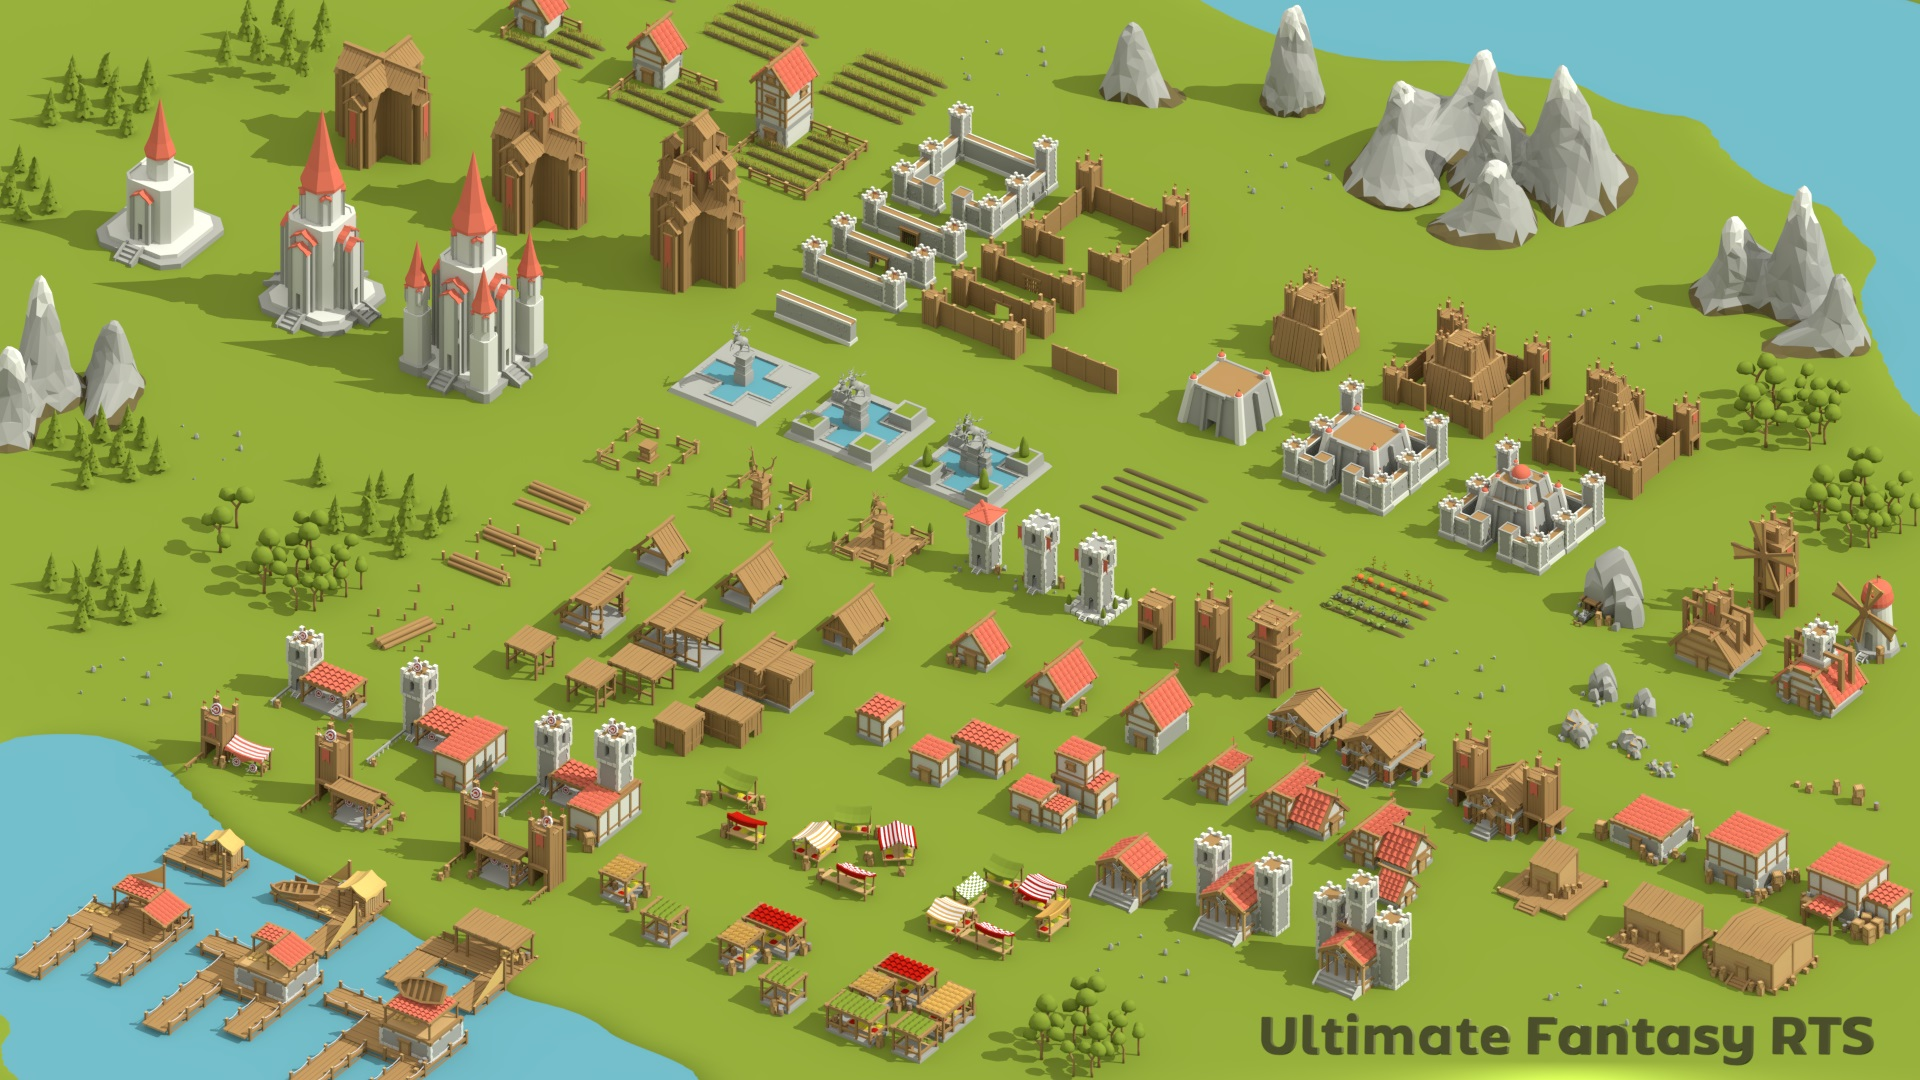
\includegraphics[width=0.5\linewidth]{images/assets.png}
    \caption{Exemples d'assets low poly utilisés}
    \label{fig:assets}
\end{figure}

Ces assets ont été intégrés dans le moteur de jeu.

\paragraph{Limites et perspectives}

Même si cette solution nous a permis de gagner un temps considérable, elle présente certaines limites. Tout d’abord, le style visuel du jeu dépend actuellement de ressources externes que nous ne maîtrisons pas totalement. Ensuite, l’uniformité graphique peut parfois être compromise si les assets proviennent de sources différentes. Enfin, l’utilisation de modèles génériques réduit la capacité à représenter


